In this section is presented the detailed alloy specification for the system, as outlined and described in the RASD. \\

\lstinputlisting[language=alloy]{Alloy/Alloy.als}
\newpage

\begin{figure}[H]
    \begin{center}
        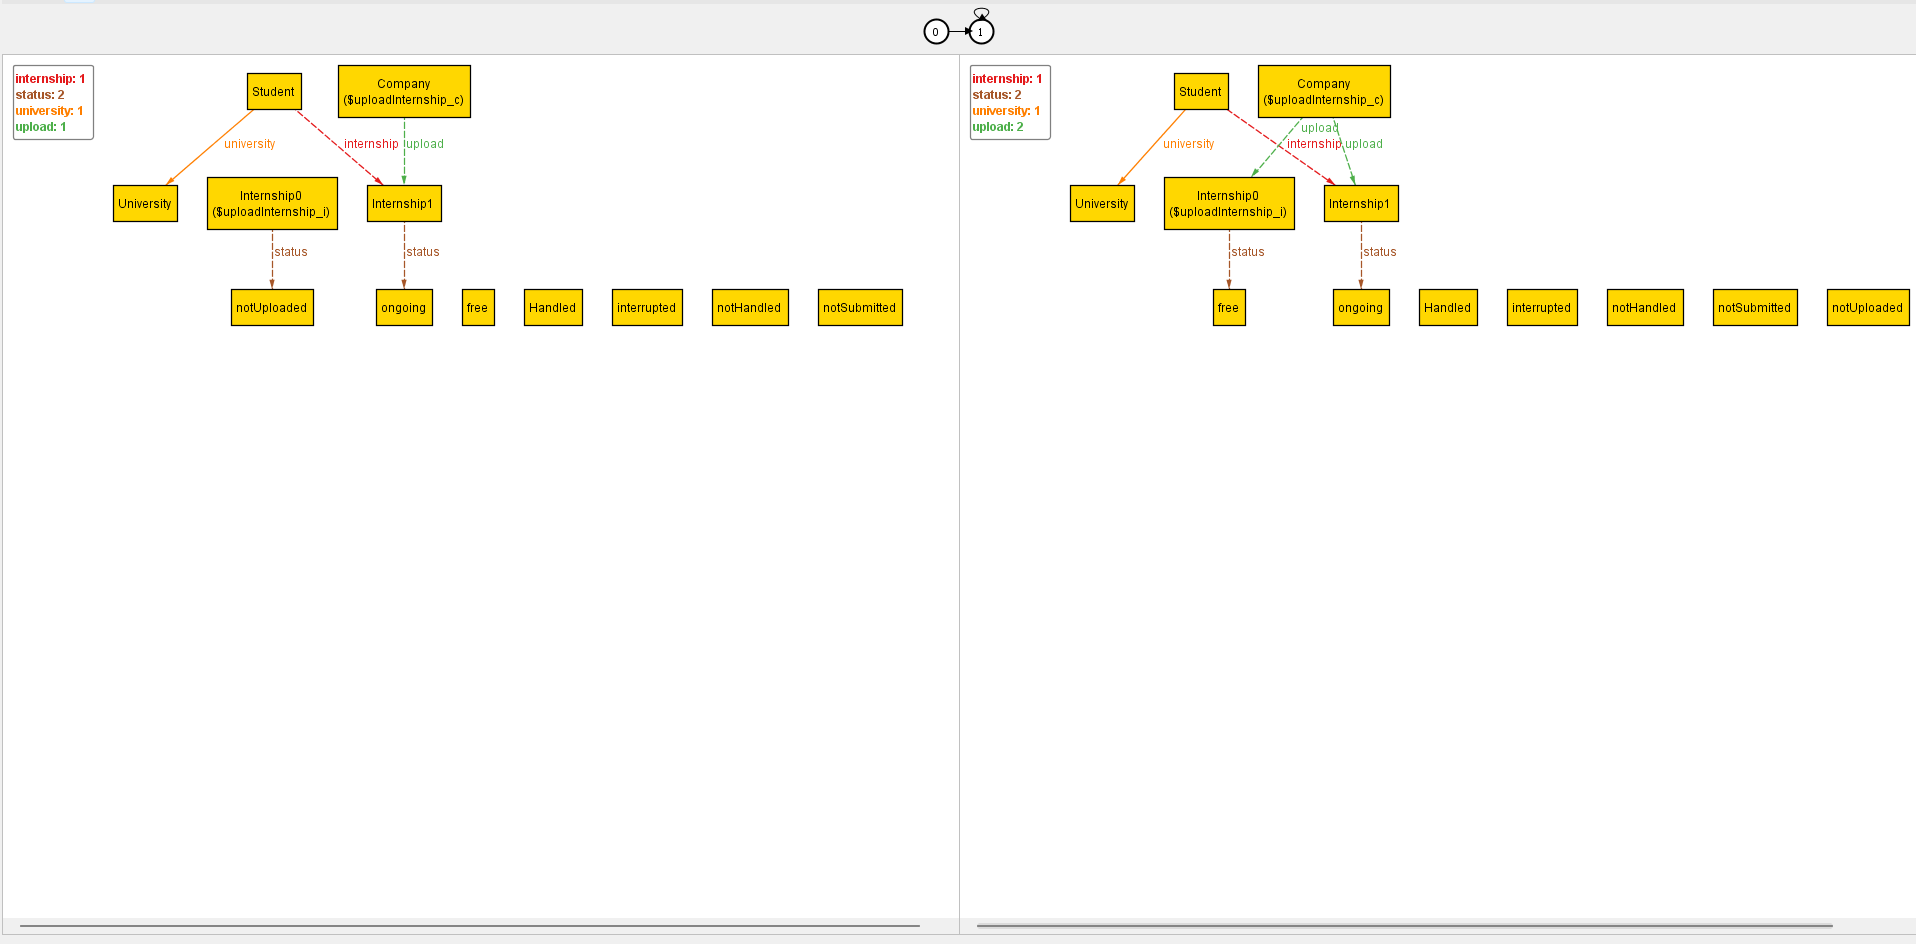
\includegraphics[width=\linewidth]{Images/Alloy/uploadInternship.png}
        \caption{Example of the predicate uploadInternship.}
        \label{fig:upload_intern_alloy}%
    \end{center}
\end{figure}

\begin{figure}[H]
    \begin{center}
        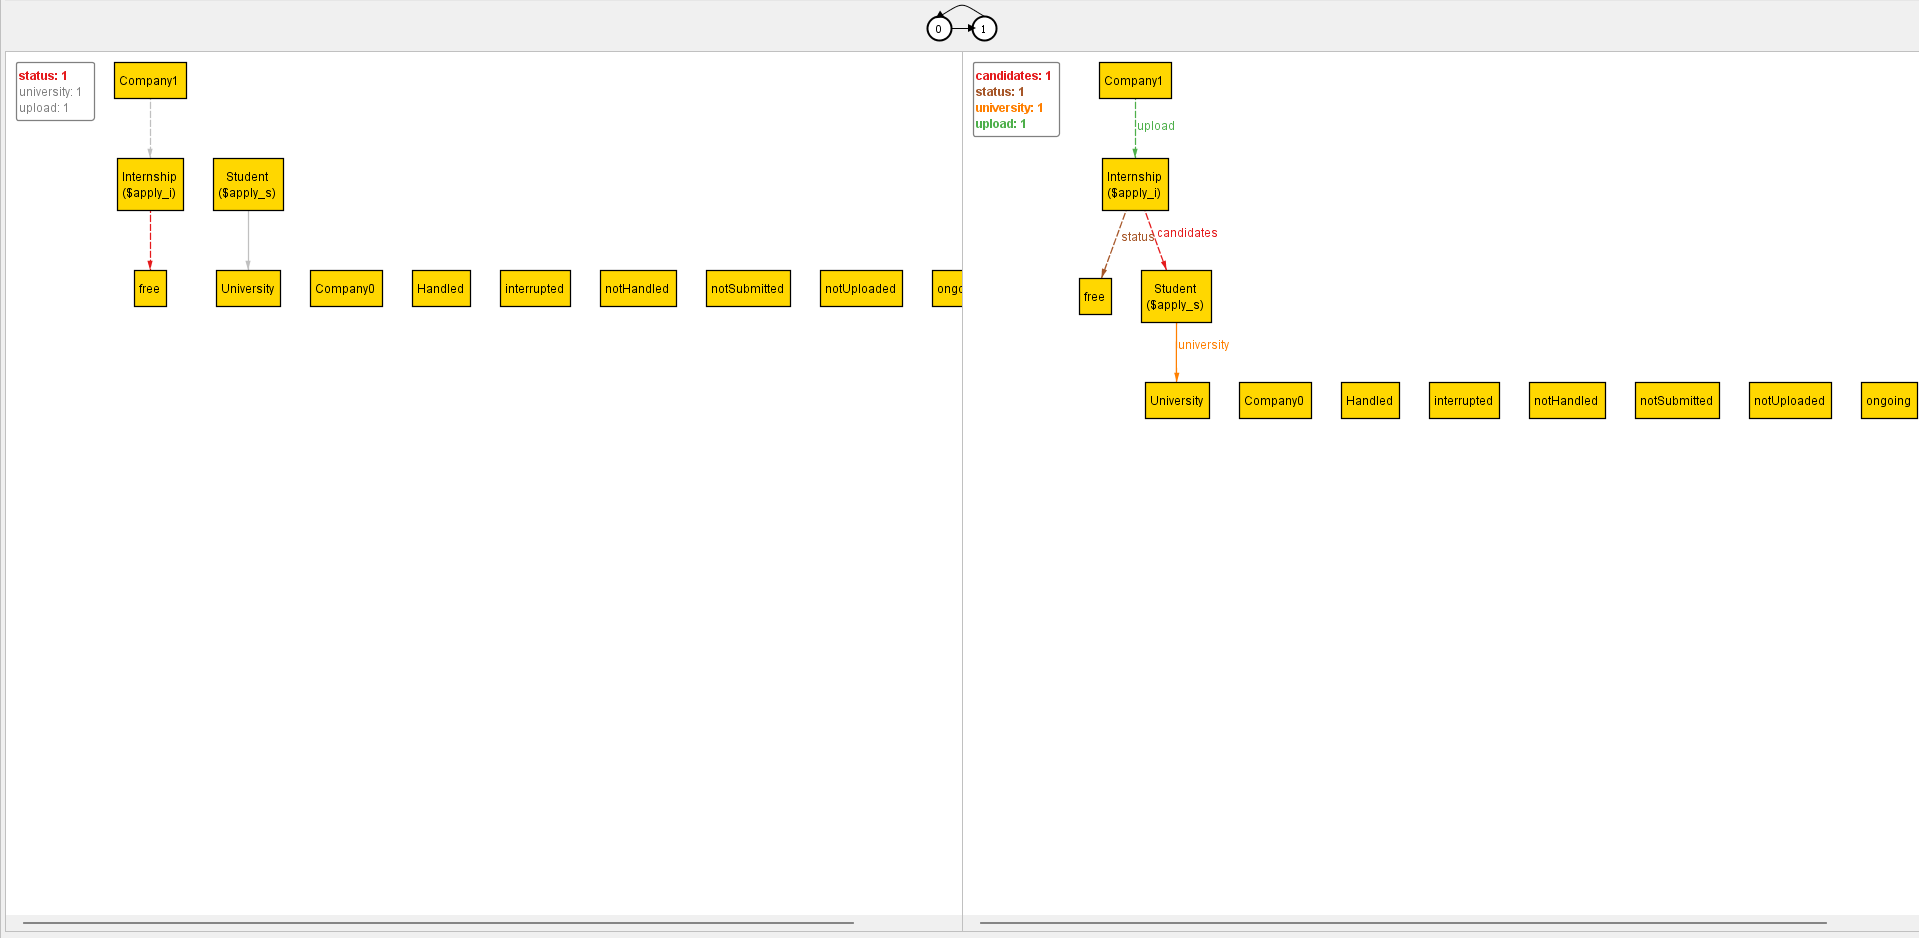
\includegraphics[width=\linewidth]{Images/Alloy/apply.png}
        \caption{Example of the predicate apply.}
        \label{fig:apply_alloy}%
    \end{center}
\end{figure}


\begin{figure}[H]
    \begin{center}
        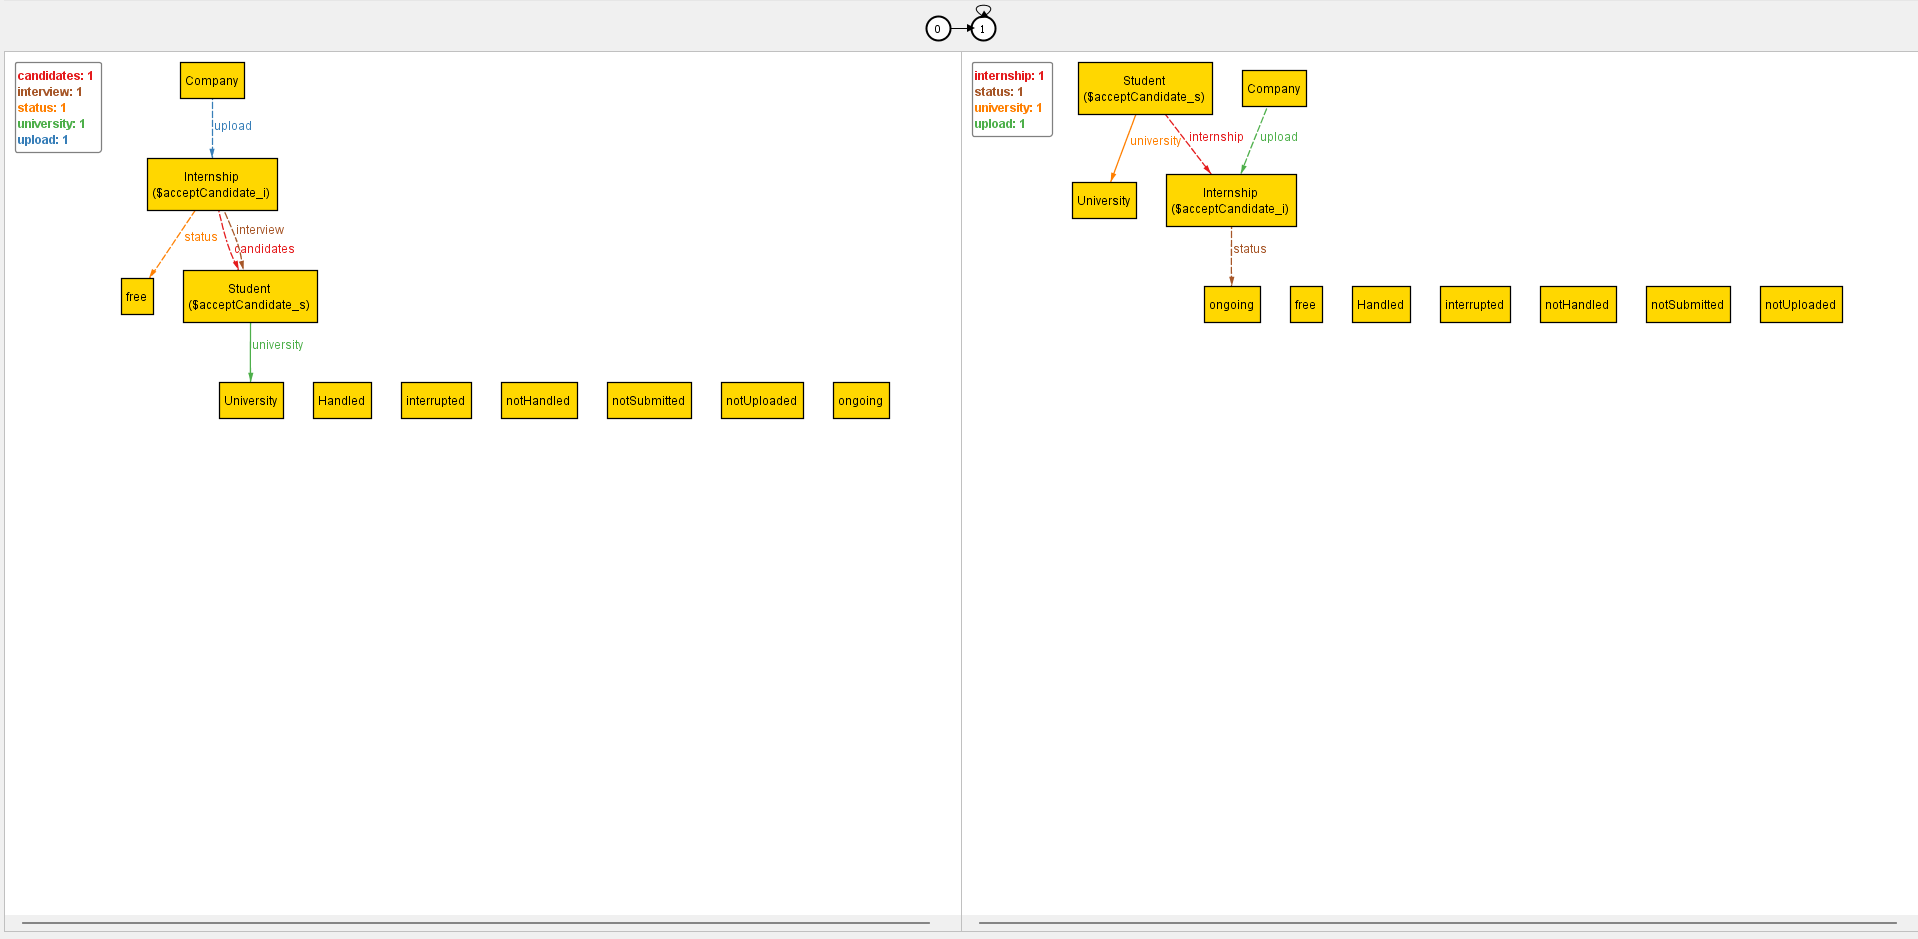
\includegraphics[width=\linewidth]{Images/Alloy/acceptCandidate.png}
        \caption{Example of the predicate acceptCandidate.}
        \label{fig:accept_candidate_alloy}%
    \end{center}
\end{figure}

\begin{figure}[H]
    \begin{center}
        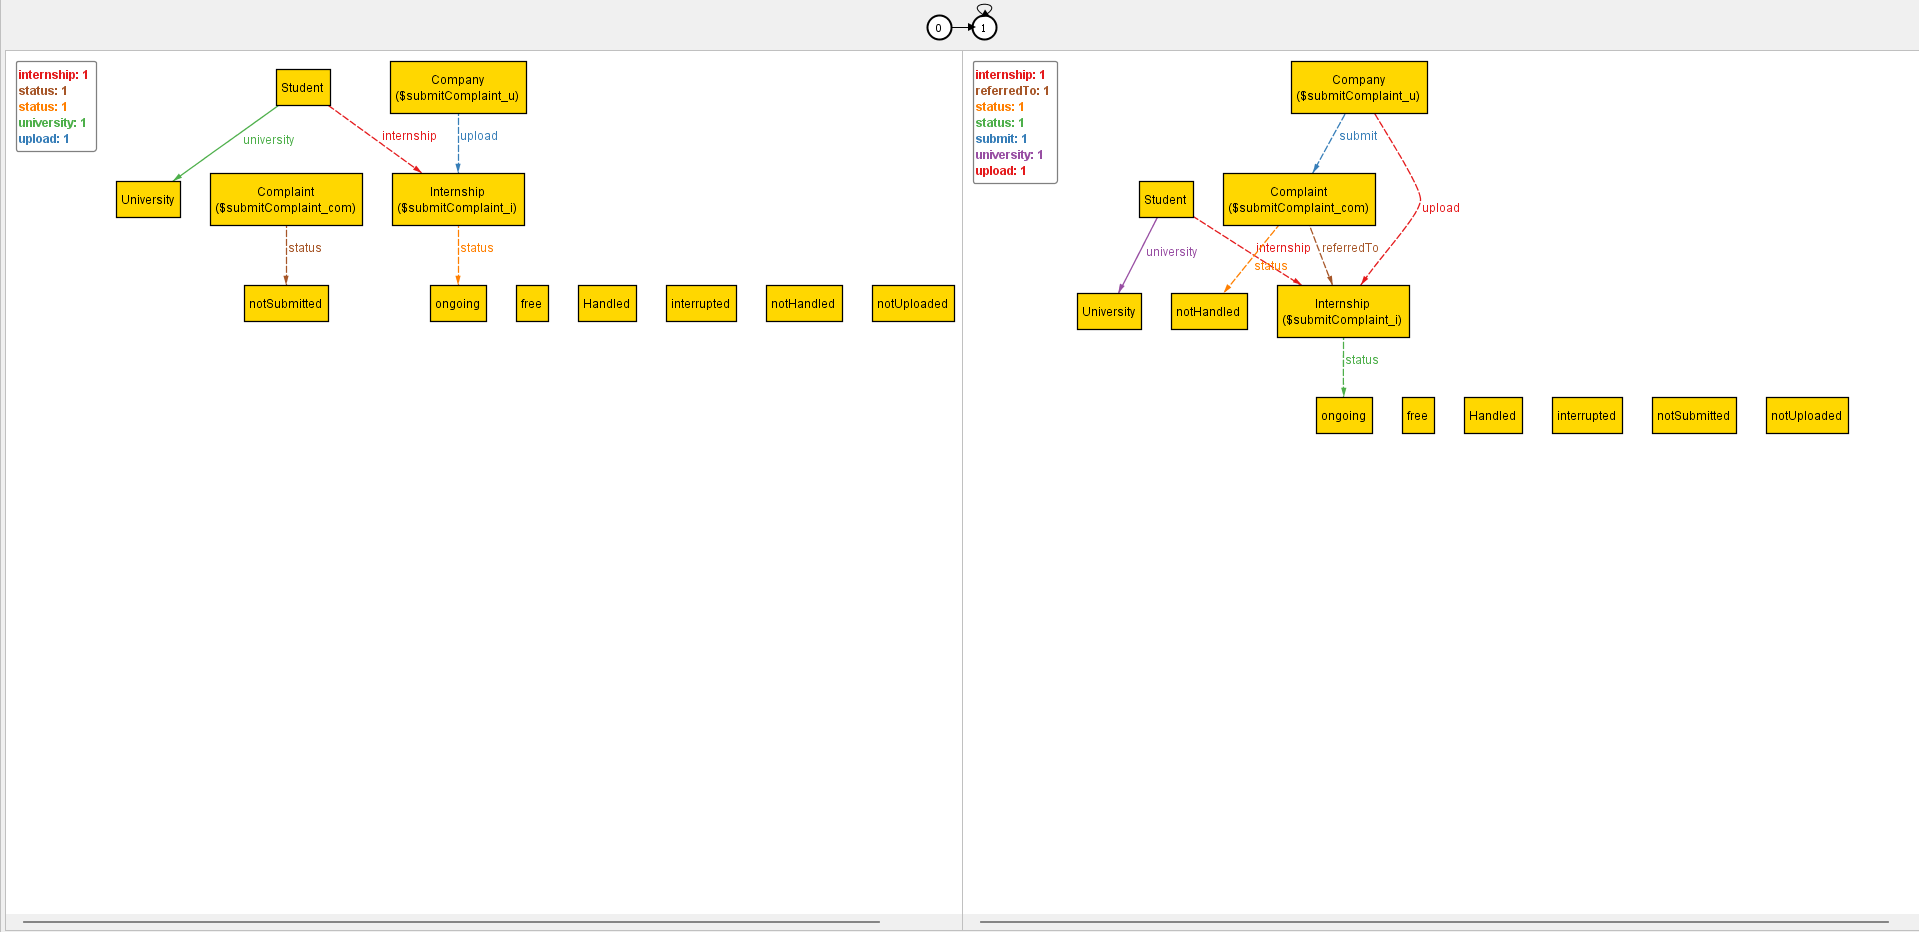
\includegraphics[width=\linewidth]{Images/Alloy/submitComplaint.png}
        \caption{Example of the predicate submitComplaint.}
        \label{fig:submit_complaint_alloy}%
    \end{center}
\end{figure}

\begin{figure}[H]
    \begin{center}
        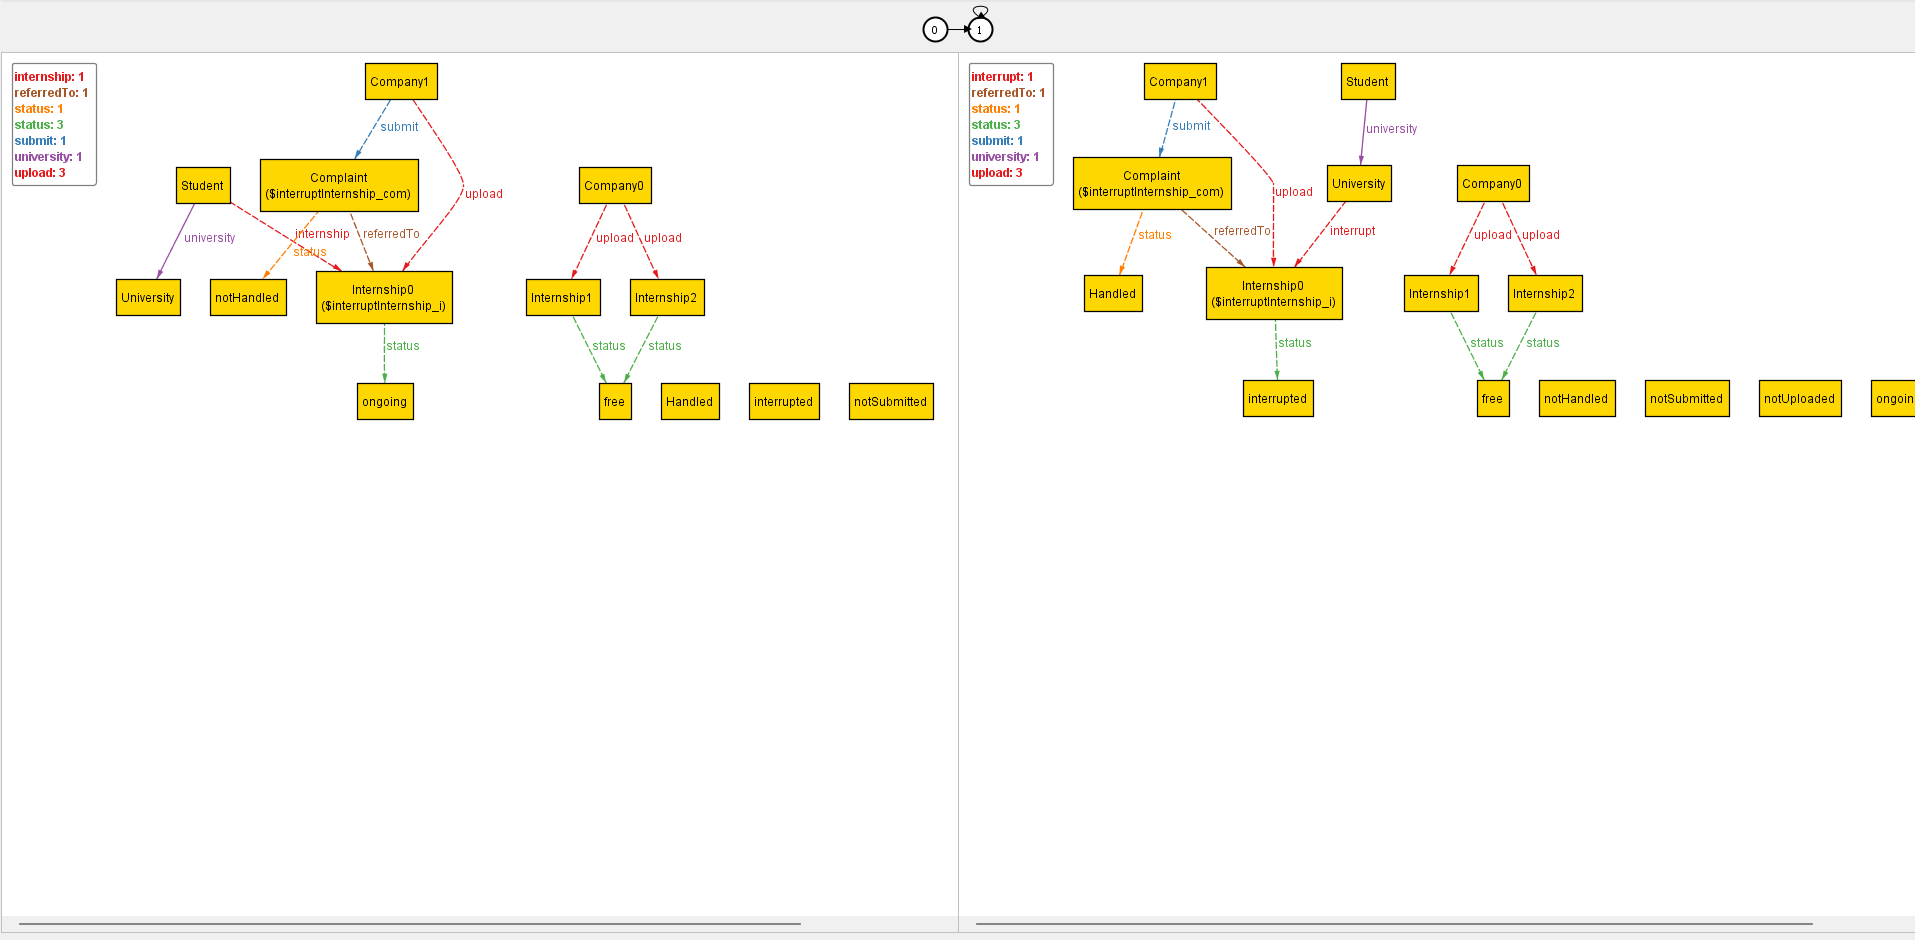
\includegraphics[width=\linewidth]{RASD//Images//Alloy/interruptInternship.png}
        \caption{Example of the predicate interruptInternship.}
        \label{fig:schedule_intern_alloy}%
    \end{center}
\end{figure}

\begin{figure}[H]
    \begin{center}
        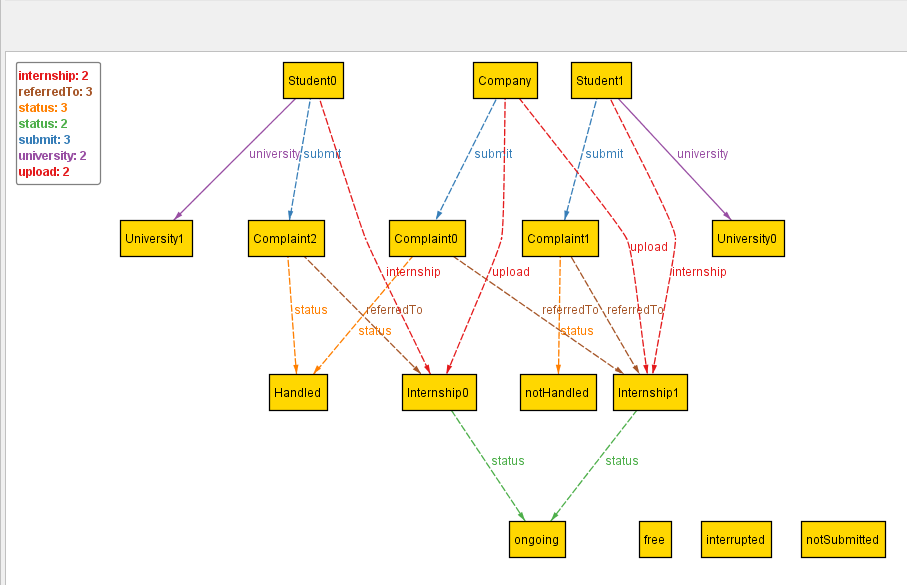
\includegraphics[width=\linewidth]{RASD//Images//Alloy/show.png}
        \caption{Example of a possible world by running predicate Show.}
        \label{fig:show_world_alloy}%
    \end{center}
\end{figure}